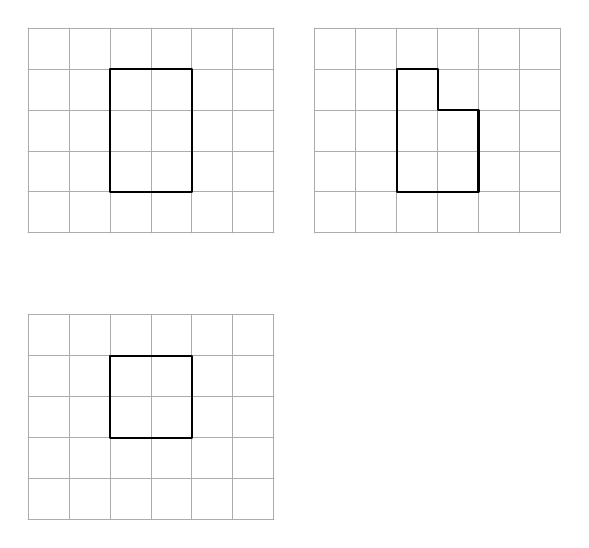
\begin{tikzpicture}[line cap=round,line join=round,line width=0.8pt,scale=0.52]
\begin{scope}[shift={(0,3)}]
  \draw[gray!65,line width=0.35pt] (0,0) grid (6,5);
  \draw[black] (2,1)--(4,1)--(4,4)--(2,4)--cycle;
\end{scope}
\begin{scope}[shift={(7,3)}]
  \draw[gray!65,line width=0.35pt] (0,0) grid (6,5);
  \draw[black] (2,1)--(4,1)--(4,3)--(3,3)--(3,4)--(2,4)--cycle;
\end{scope}
\begin{scope}[shift={(0,-4)}]
  \draw[gray!65,line width=0.35pt] (0,0) grid (6,5);
  \draw[black] (2,2)--(4,2)--(4,4)--(2,4)--cycle;
\end{scope}
\end{tikzpicture}
